\chapter{Os íons e as soluções iônicas}\label{ch:g9:ions}

Duas bebidas límpidas estão num banco de academia: uma garrafa de bebida
isotônica, vendida pelos seus ``eletrólitos'', e um copo de água com
açúcar. Num laboratório, duas placas de metal ligadas a uma pilha e a
uma lâmpada pequena são mergulhadas em cada uma, uma de cada vez. Na
bebida isotônica, a lâmpada acende; na água com açúcar, ela continua
apagada. Alguma coisa no primeiro líquido transporta carga elétrica, e o
açúcar não. Essa alguma coisa são os \omterm{def:g9:ions:ion}{íons}.

\begin{recall}
Um \omterm{def:g7:atoms-and-molecules:atom}{átomo} tem um \omterm{def:g9:inside-the-atom:nucleus}{núcleo} com $Z$ \omterm{def:g9:inside-the-atom:proton}{prótons}, cada um de carga $+e$, e $Z$
\omterm{def:g9:inside-the-atom:nucleus}{elétrons} em volta dele, cada um de carga $-e$: o \omterm{def:g7:atoms-and-molecules:atom}{átomo} é neutro
(\cref{ch:g9:inside-the-atom}). Um \omterm{def:g6:solutions-and-solubility:solute}{soluto} dissolvido na água dá uma
\omterm{def:g6:solutions-and-solubility:solute}{solução aquosa} (\cref{ch:g6:solutions-and-solubility}). Um \omterm{def:g7:identifying-substances:characteristic-test}{teste
característico} detecta uma espécie por um resultado visível
(\cref{ch:g7:identifying-substances}).
\end{recall}

\begin{omfigure}
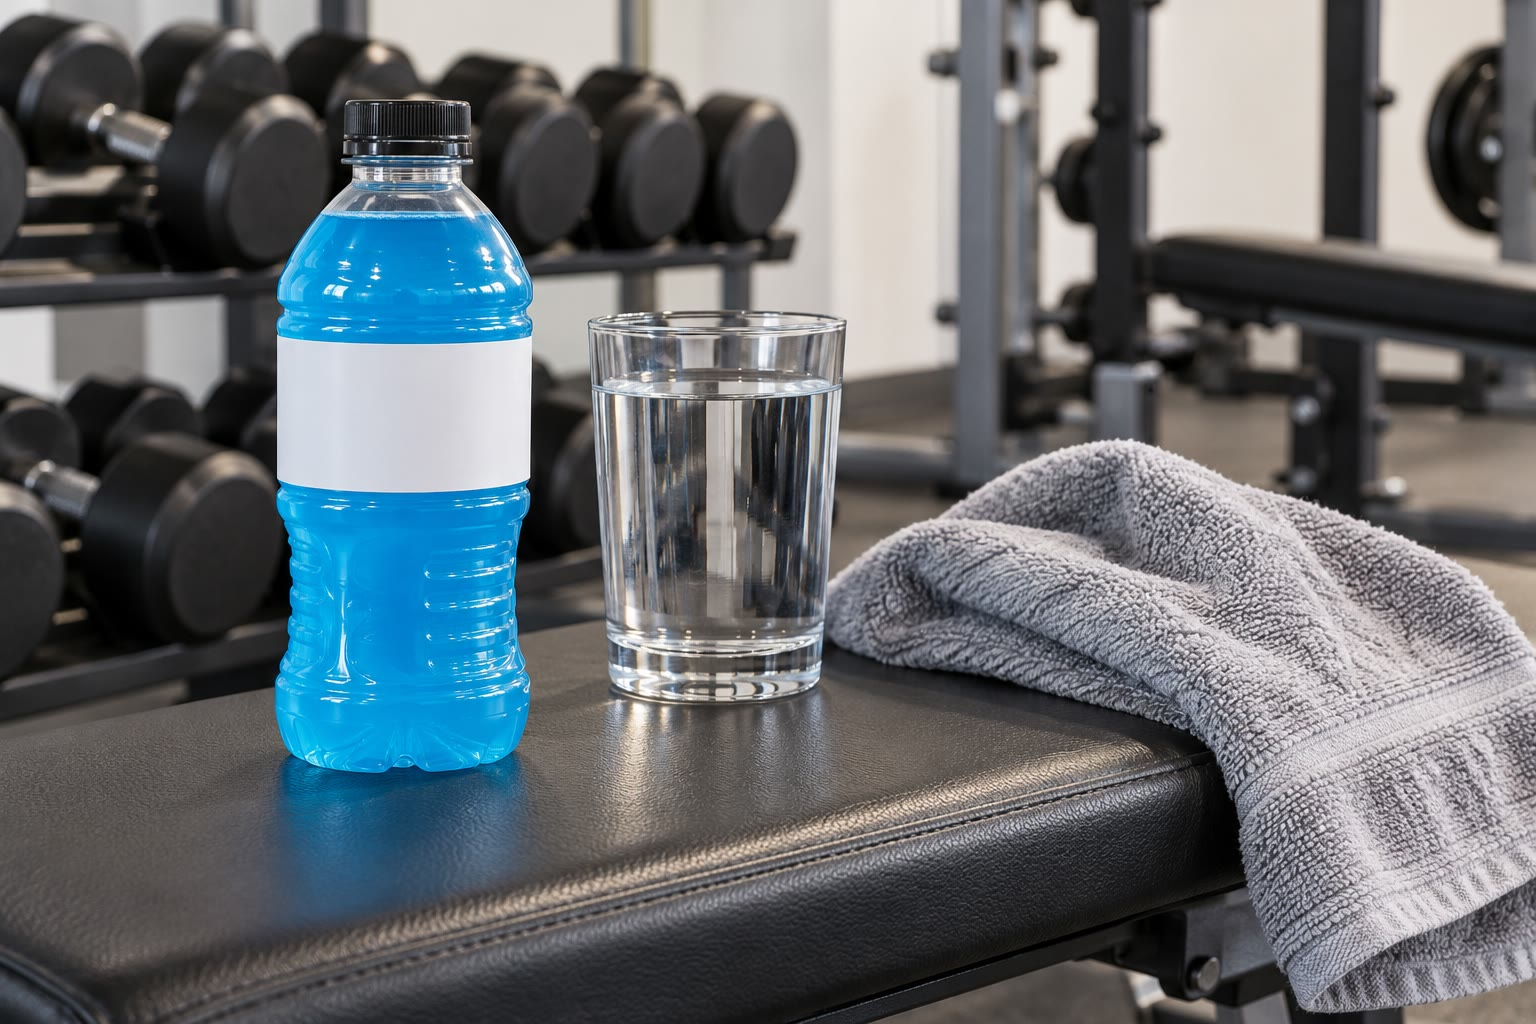
\includegraphics[width=0.5\linewidth]{images/book1/ai/g9-sports-drink.jpg}

{\small Uma bebida isotônica e um copo de água: a bebida contém \omterm{def:g9:ions:ion}{íons}
dissolvidos.}
\end{omfigure}

\section{Átomos que ganham ou perdem elétrons}

\begin{definition}[Íon, cátion, ânion]\label{def:g9:ions:ion}
Um \emph{íon}\index{ion@íon} é um \omterm{def:g7:atoms-and-molecules:atom}{átomo}, ou um grupo de \omterm{def:g7:atoms-and-molecules:atom}{átomos}, que perdeu ou
ganhou um ou mais \omterm{def:g9:inside-the-atom:nucleus}{elétrons} e, por isso, tem carga elétrica. Um íon de
carga positiva, que perdeu \omterm{def:g9:inside-the-atom:nucleus}{elétrons}, é um \emph{cátion}\index{cation@cátion};
um íon de carga negativa, que ganhou \omterm{def:g9:inside-the-atom:nucleus}{elétrons}, é um
\emph{ânion}\index{anion@ânion}. A carga é escrita no alto, à direita da
fórmula: \ce{Na+}, \ce{Cu^{2+}}, \ce{Cl-}.
\end{definition}

\begin{example}[O sódio e o cloro]\label{ex:g9:ions:na-cl}
Um \omterm{def:g7:atoms-and-molecules:atom}{átomo} de sódio, 11 \omterm{def:g9:inside-the-atom:proton}{prótons} e 11 \omterm{def:g9:inside-the-atom:nucleus}{elétrons}, perde um \omterm{def:g9:inside-the-atom:nucleus}{elétron}: ele vira
o \omterm{def:g9:ions:ion}{íon} sódio \ce{Na+}, 11 \omterm{def:g9:inside-the-atom:proton}{prótons} e 10 \omterm{def:g9:inside-the-atom:nucleus}{elétrons}, carga
$+1$:
\[
  \ce{Na -> Na+ + e-}.
\]
Um \omterm{def:g7:atoms-and-molecules:atom}{átomo} de cloro, 17 \omterm{def:g9:inside-the-atom:proton}{prótons} e 17 \omterm{def:g9:inside-the-atom:nucleus}{elétrons}, ganha um \omterm{def:g9:inside-the-atom:nucleus}{elétron}: ele vira
o \omterm{def:g9:ions:ion}{íon} cloreto \ce{Cl-}, 17 \omterm{def:g9:inside-the-atom:proton}{prótons} e 18 \omterm{def:g9:inside-the-atom:nucleus}{elétrons}:
\[
  \ce{Cl + e- -> Cl-}.
\]
\end{example}

\begin{omfigure}
\begin{tikzpicture}[font=\small]
  \foreach \x/\name/\p/\e/\ch/\col in {0/{átomo de sódio}/11/11/0/omDef,
      3.7/{íon sódio\\ \ce{Na+}}/11/10/+1/omProp,
      8.0/{átomo de cloro}/17/17/0/omDef, 11.7/{íon cloreto\\ \ce{Cl-}}/17/18/$-1$/omProp} {
    \node[draw=\col, fill=\col!6, rounded corners=2pt, align=center, text width=2.4cm]
      at (\x,0) {\textbf{\name}\\ \p\ prótons\\ \e\ elétrons\\ carga \ch};
  }
  \draw[->, thick, omProp] (1.45,0) -- (2.25,0) node[midway, above, text=black,
    font=\footnotesize, align=center] {perde\\ 1 \ce{e-}};
  \draw[->, thick, omProp] (9.45,0) -- (10.25,0) node[midway, above, text=black,
    font=\footnotesize, align=center] {ganha\\ 1 \ce{e-}};
\end{tikzpicture}

{\small Um \omterm{def:g7:atoms-and-molecules:atom}{átomo} de sódio vira um \omterm{def:g9:ions:ion}{íon} sódio perdendo um \omterm{def:g9:inside-the-atom:nucleus}{elétron}; um \omterm{def:g7:atoms-and-molecules:atom}{átomo}
de cloro vira um \omterm{def:g9:ions:ion}{íon} cloreto ganhando um. Os \omterm{def:g9:inside-the-atom:proton}{prótons} não mudam.}
\end{omfigure}

\begin{proposition}[Alguns íons comuns]\label{prop:g9:ions:common}
Os \omterm{def:g9:ions:ion}{íons} monoatômicos são formados a partir de um \omterm{def:g7:atoms-and-molecules:atom}{átomo}; os \omterm{def:g9:ions:ion}{íons}
poliatômicos, a partir de um grupo de \omterm{def:g7:atoms-and-molecules:atom}{átomos} que fica junto:
\begin{center}
\small
\begin{tabular}{llll}
\hline
\omterm{def:g9:ions:ion}{cátions} & & \omterm{def:g9:ions:ion}{ânions} & \\
\hline
sódio & \ce{Na+} & cloreto & \ce{Cl-} \\
potássio & \ce{K+} & hidróxido & \ce{OH-} \\
cálcio & \ce{Ca^{2+}} & nitrato & \ce{NO3-} \\
magnésio & \ce{Mg^{2+}} & carbonato & \ce{CO3^{2-}} \\
cobre(II) & \ce{Cu^{2+}} & sulfato & \ce{SO4^{2-}} \\
ferro(II), ferro(III) & \ce{Fe^{2+}}, \ce{Fe^{3+}} & & \\
zinco & \ce{Zn^{2+}} & & \\
alumínio & \ce{Al^{3+}} & & \\
amônio & \ce{NH4+} & & \\
\hline
\end{tabular}
\end{center}
\end{proposition}

\section{Os compostos iônicos e as suas fórmulas}

\begin{definition}[Composto iônico]\label{def:g9:ions:ionic-compound}
Um \emph{composto iônico}\index{composto ionico@composto iônico} é formado por \omterm{def:g9:ions:ion}{cátions} e
\omterm{def:g9:ions:ion}{ânions} em números tais que o conjunto não tem carga. A sua fórmula dá a
proporção dos \omterm{def:g9:ions:ion}{íons}, sem as cargas: \ce{NaCl} para o cloreto de sódio, um
\ce{Na+} para cada \ce{Cl-}; \ce{CaCl2} para o cloreto de cálcio, dois
\ce{Cl-} para cada \ce{Ca^{2+}}.
\end{definition}

\begin{method}[Escrever a fórmula de um composto iônico]\label{met:g9:ions:formula}
\begin{enumerate}
  \item Escreva os dois \omterm{def:g9:ions:ion}{íons} com as suas cargas, primeiro o \omterm{def:g9:ions:ion}{cátion}.
  \item Encontre os menores números de cada um que tornam a carga total
        nula.
  \item Escreva esses números como \omterm{def:g7:atoms-and-molecules:formula}{índices}; um \omterm{def:g9:ions:ion}{íon} poliatômico que
        precisa de \omterm{def:g7:atoms-and-molecules:formula}{índice} vai entre parênteses.
\end{enumerate}
Óxido de alumínio: \ce{Al^{3+}} e \ce{O^{2-}}; $2 \times (+3) + 3 \times
(-2) = 0$, logo \ce{Al2O3}. Hidróxido de ferro(III): \ce{Fe^{3+}} e três
\ce{OH-}: \ce{Fe(OH)3}.
\end{method}

\begin{proposition}[Um sólido iônico é um empilhamento de íons]\label{prop:g9:ions:solid}
Num cristal de sal, os \omterm{def:g9:ions:ion}{íons} sódio e os \omterm{def:g9:ions:ion}{íons} cloreto se alternam num
empilhamento regular em três dimensões, cada \omterm{def:g9:ions:ion}{íon} cercado por \omterm{def:g9:ions:ion}{íons} de
carga oposta, que o mantêm no lugar. Um grão de sal de cozinha contém
bilhões de bilhões deles; a sua forma cúbica reflete o empilhamento
cúbico.
\end{proposition}

\begin{omfigure}
\begin{minipage}[b]{0.5\linewidth}\centering
\begin{tikzpicture}[font=\small]
  \foreach \i in {0,...,5} \foreach \j in {0,...,4} {
    \pgfmathtruncatemacro\pp{mod(\i+\j,2)}
    \ifnum\pp=0 \node[aNa, minimum size=5mm] at (0.62*\i,0.62*\j) {};
    \else \node[aCl, minimum size=7.4mm] at (0.62*\i,0.62*\j) {};\fi
  }
\end{tikzpicture}

{\small Uma camada de um cristal de sal: os \omterm{def:g9:ions:ion}{íons} sódio (roxos, menores) e
os \omterm{def:g9:ions:ion}{íons} cloreto (verdes) se alternam.}
\end{minipage}\hfill
\begin{minipage}[b]{0.3\linewidth}\centering
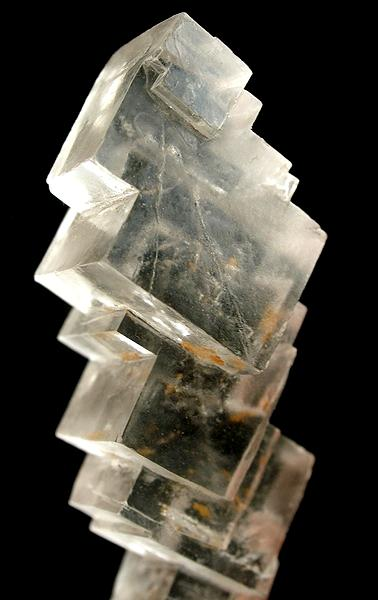
\includegraphics[height=4.6cm]{images/book1/halite.jpg}

{\small A halita, sal-gema natural. Foto: Robert M.~Lavinsky,
CC BY-SA 3.0.}
\end{minipage}
\end{omfigure}

\section{As soluções iônicas conduzem}

\begin{notation}[O símbolo de estado (aq)]\label{not:g9:ions:aq}
Um \omterm{def:g9:ions:ion}{íon} ou uma \omterm{def:g7:atoms-and-molecules:molecule}{molécula} dissolvidos em água são marcados com (aq), de
aquoso: \ce{Na+(aq)}, \ce{Cl-(aq)}.
\end{notation}

\begin{proposition}[As soluções iônicas conduzem a eletricidade]\label{prop:g9:ions:conduct}
Quando um \omterm{def:g9:ions:ionic-compound}{composto iônico} \omterm{def:g2:mixing-and-dissolving:dissolve}{se dissolve} na água, os seus \omterm{def:g9:ions:ion}{íons} se separam e
se movem livremente na solução: a água salgada contém \ce{Na+(aq)} e
\ce{Cl-(aq)}. \omterm{def:g9:ions:ion}{Íons} em movimento transportam carga elétrica, por isso uma
solução iônica conduz a eletricidade. Uma solução de açúcar, cujas
\omterm{def:g7:atoms-and-molecules:molecule}{moléculas} não têm carga, não conduz; nem a água muito pura.
\end{proposition}

\begin{inthelab}[Que líquidos conduzem?]
O professor liga num circuito duas placas de metal, uma pilha de baixa
tensão e uma lâmpada pequena; as placas são mergulhadas, uma vez em
cada, em água destilada, água com açúcar, água salgada e numa solução de
sulfato de cobre, e enxaguadas entre uma e outra. A lâmpada só acende
com as duas soluções iônicas.
\end{inthelab}

\begin{omfigure}
\begin{tikzpicture}[font=\small, scale=1.1]
  \foreach \xs/\lit/\lab in {0/1/{água salgada: a lâmpada acende}, 5.2/0/{água com açúcar: ela fica apagada}} {
    \begin{scope}[xshift=\xs cm]
      \pic[transform shape] at (2,0) {beaker={0.7}{omWater!80}};
      \fill[black!45] (1.6,0.25) rectangle (1.7,2.6);
      \fill[black!45] (2.3,0.25) rectangle (2.4,2.6);
      \ifnum\lit=1 \fill[yellow!70, opacity=0.8] (3.4,3.0) circle (0.42);\fi
      \draw (1.65,2.6) -- (1.65,3.6) to[battery1] (3.4,3.6) -- (3.4,3.4)
        to[lamp] (3.4,2.6) -- (2.35,2.6);
      \node[anchor=north, align=center] at (2,-0.15) {\lab};
    \end{scope}
  }
\end{tikzpicture}

{\small O teste de condutividade: com a água salgada, os \omterm{def:g9:ions:ion}{íons}
transportam a corrente e a lâmpada acende; a água com açúcar não contém
\omterm{def:g9:ions:ion}{íons}, e a lâmpada continua apagada.}
\end{omfigure}

\section{Testes de precipitação para os íons}

\begin{definition}[Precipitado]\label{def:g9:ions:precipitate}
Quando duas soluções são \omterm{def:g2:mixing-and-dissolving:mix}{misturadas}, um \omterm{def:g9:ions:ion}{cátion} de uma e um \omterm{def:g9:ions:ion}{ânion} da
outra podem formar um \omterm{def:g9:ions:ionic-compound}{composto iônico} que não \omterm{def:g2:mixing-and-dissolving:dissolve}{se dissolve}. Ele aparece
como um sólido fino que turva o líquido e se deposita: um
\emph{precipitado}\index{precipitado}. A reação é uma
\emph{precipitação}\index{precipitacao@precipitação}.
\end{definition}

\begin{proposition}[Testes para íons comuns]\label{prop:g9:ions:tests}
Algumas gotas de uma solução de \omterm{def:g7:chemical-reactions:reactant}{reagente} identificam um \omterm{def:g9:ions:ion}{íon} pela cor do
\omterm{def:g9:ions:precipitate}{precipitado} que ele forma:
\begin{center}
\small
\begin{tabular}{llll}
\hline
\omterm{def:g9:ions:ion}{íon} procurado & \omterm{def:g7:chemical-reactions:reactant}{reagente} & \omterm{def:g9:ions:precipitate}{precipitado} & cor \\
\hline
cobre(II) \ce{Cu^{2+}} & hidróxido de sódio & \ce{Cu(OH)2} & azul \\
ferro(II) \ce{Fe^{2+}} & hidróxido de sódio & \ce{Fe(OH)2} & verde \\
ferro(III) \ce{Fe^{3+}} & hidróxido de sódio & \ce{Fe(OH)3} & castanho-alaranjado \\
zinco \ce{Zn^{2+}} & hidróxido de sódio & \ce{Zn(OH)2} & branco \\
alumínio \ce{Al^{3+}} & hidróxido de sódio & \ce{Al(OH)3} & branco \\
cloreto \ce{Cl-} & nitrato de prata & \ce{AgCl} & branco, escurece à luz \\
\hline
\end{tabular}
\end{center}
\end{proposition}

\begin{example}[Escrever uma precipitação]\label{ex:g9:ions:equation}
Só são escritos os \omterm{def:g9:ions:ion}{íons} que formam o sólido; os outros continuam
dissolvidos e não participam:
\[
  \ce{Cu^{2+}(aq) + 2OH-(aq) -> Cu(OH)2(s)}, \qquad
  \ce{Ag+(aq) + Cl-(aq) -> AgCl(s)}.
\]
\end{example}
\begin{omfigure}
\begin{tikzpicture}[font=\small, scale=0.95]
  \foreach \k/\pc/\lab in {0/blue!60/{\ce{Cu^{2+}}: azul}, 1/green!45!black!70/{\ce{Fe^{2+}}: verde},
      2/orange!70!brown/{\ce{Fe^{3+}}: castanho-\\alaranjado}, 3/white!85!black/{\ce{Zn^{2+}}: branco},
      4/white!85!black/{\ce{Al^{3+}}: branco}, 5/white!80!black/{\ce{Cl-}: branco}} {
    \pic[transform shape] at (\k*2.3,0) {testtube={0.5}{omWater!60}};
    \pic[transform shape] at (\k*2.3,0) {testtube={0.14}{\pc}};
    \node[anchor=north, align=center, font=\footnotesize, text width=2cm] at (\k*2.3,-0.15) {\lab};
  }
\end{tikzpicture}

{\small \omterm{def:g9:ions:precipitate}{Precipitados} formados com hidróxido de sódio (os cinco primeiros
tubos) e com nitrato de prata (o último tubo).}
\end{omfigure}

\begin{safety}{\ghs[0.82cm]{GHS05}\ghs[0.82cm]{GHS07}}
% ledger: ghs:NaOH, ghs:AgNO3
Hidróxido de sódio: provoca queimaduras graves na pele e lesões nos
olhos, e pode ser corrosivo para os metais (GHS05); irritante para a
pele e os olhos quando diluído (GHS07). O nitrato de prata, o \omterm{def:g7:chemical-reactions:reactant}{reagente}
do cloreto, é oxidante, corrosivo e muito tóxico para os organismos
aquáticos. Óculos de proteção, luvas; \omterm{def:g7:chemical-reactions:reactant}{reagentes} distribuídos gota a gota
pelo professor.
\end{safety}

\begin{method}[Testar um íon]\label{met:g9:ions:test}
\begin{enumerate}
  \item Despeje um pouco da solução a ser testada num tubo de ensaio.
  \item Acrescente o \omterm{def:g7:chemical-reactions:reactant}{reagente} gota a gota.
  \item Anote a cor do \omterm{def:g9:ions:precipitate}{precipitado}, se houver, e compare com a tabela.
  \item Conclua, e lembre-se de que um teste identifica um \omterm{def:g9:ions:ion}{íon}, não um
        composto: a solução de cloreto de ferro(III) dá ao mesmo tempo o
        teste do \ce{Fe^{3+}} e o teste do \ce{Cl-}.
\end{enumerate}
\end{method}

\section{Exercícios}

\begin{exercise}[$\star$]\label{exo:g9:ions:1}
O que é um \omterm{def:g9:ions:ion}{íon}? Qual é a diferença entre um \omterm{def:g9:ions:ion}{cátion} e um \omterm{def:g9:ions:ion}{ânion}?
\end{exercise}

\begin{exercise}[$\star$]\label{exo:g9:ions:2}
Um \omterm{def:g7:atoms-and-molecules:atom}{átomo} de magnésio (12 \omterm{def:g9:inside-the-atom:proton}{prótons}) perde dois \omterm{def:g9:inside-the-atom:nucleus}{elétrons}. Escreva a fórmula
do \omterm{def:g9:ions:ion}{íon} formado, e dê os números de \omterm{def:g9:inside-the-atom:proton}{prótons} e de \omterm{def:g9:inside-the-atom:nucleus}{elétrons} dele.
\end{exercise}

\begin{exercise}[$\star$]\label{exo:g9:ions:3}
Escreva as fórmulas do cloreto de potássio, do cloreto de magnésio e do
óxido de cálcio (\omterm{def:g9:ions:ion}{íon} óxido: \ce{O^{2-}}).
\end{exercise}

\begin{exercise}[$\star$]\label{exo:g9:ions:4}
Por que a água salgada conduz a eletricidade e a água com açúcar não?
\end{exercise}

\begin{exercise}[$\star\star$]\label{exo:g9:ions:5}
Escreva as fórmulas do sulfato de cobre(II), do cloreto de alumínio e do
carbonato de sódio.
\end{exercise}

\begin{exercise}[$\star\star$]\label{exo:g9:ions:6}
O hidróxido de sódio acrescentado a uma solução dá um \omterm{def:g9:ions:precipitate}{precipitado}
castanho-alaranjado. Que \omterm{def:g9:ions:ion}{íon} a solução contém? Escreva a equação da
\omterm{def:g9:ions:precipitate}{precipitação}.
\end{exercise}

\begin{exercise}[$\star\star$]\label{exo:g9:ions:7}
Quantos \omterm{def:g9:inside-the-atom:nucleus}{elétrons} o \omterm{def:g9:ions:ion}{íon} sulfato \ce{SO4^{2-}} tem a mais do que os seus
\omterm{def:g9:inside-the-atom:proton}{prótons}? E o \omterm{def:g9:ions:ion}{íon} nitrato \ce{NO3-}?
\end{exercise}

\begin{exercise}[$\star\star$]\label{exo:g9:ions:8}
Uma solução dá um \omterm{def:g9:ions:precipitate}{precipitado} branco com o nitrato de prata e um azul
com o hidróxido de sódio. Dê o nome do \omterm{def:g9:ions:ionic-compound}{composto iônico} dissolvido e
escreva a fórmula dele.
\end{exercise}

\begin{exercise}[$\star\star$]\label{exo:g9:ions:9}
Olhe a figura da camada do cristal de sal. Quantos vizinhos de carga
oposta um \omterm{def:g9:ions:ion}{íon} no meio da camada tem, dentro dessa camada?
\end{exercise}

\begin{exercise}[$\star\star$]\label{exo:g9:ions:10}
Escreva a equação da \omterm{def:g9:ions:precipitate}{precipitação} do hidróxido de ferro(II) a partir dos
\omterm{def:g9:ions:ion}{íons} \ce{Fe^{2+}} e \ce{OH-}.
\end{exercise}

\begin{exercise}[$\star\star\star$]\label{exo:g9:ions:11}
Um pó branco pode ser cloreto de zinco ou cloreto de sódio. Dissolvido
na água, ele dá um \omterm{def:g9:ions:precipitate}{precipitado} branco com o hidróxido de sódio. Qual é
ele? Escreva a equação.
\end{exercise}

\begin{exercise}[$\star\star\star$]\label{exo:g9:ions:12}
Num cristal de cloreto de cálcio, quantos \omterm{def:g9:ions:ion}{íons} cloreto há para 1000
\omterm{def:g9:ions:ion}{íons} cálcio? Verifique que o cristal é neutro.
\end{exercise}

\section{Problema: o poço enferrujado}

\begin{problem}[{Problema de fim de semana --- manchas alaranjadas na pia
de um sítio, dois testes e o número de íons ferro num litro de água de
poço}]
\label{pb:g9:ions:1}
A água do poço de um sítio deixa manchas alaranjadas na pia. Um
laboratório recebe uma amostra. Recém-tirada, a água é límpida; com o
hidróxido de sódio, ela dá um \omterm{def:g9:ions:precipitate}{precipitado} verde, que fica
castanho-alaranjado em menos de uma hora na superfície, onde encontra o
\omterm{def:g4:air-a-mixture-of-gases:air}{ar}. O laboratório mede \qty{0.30}{mg} de ferro, na forma de \omterm{def:g9:ions:ion}{íons} ferro,
por litro. Tome a massa de um \omterm{def:g9:inside-the-atom:proton}{núcleon} como \qty{1.67e-27}{kg}, e 56
\omterm{def:g9:inside-the-atom:proton}{núcleons} para um \omterm{def:g7:atoms-and-molecules:atom}{átomo} de ferro.

\medskip
\noindent\textbf{Parte I --- Os testes.}
\begin{enumerate}
  \item Que \omterm{def:g9:ions:ion}{íon} o \omterm{def:g9:ions:precipitate}{precipitado} verde mostra? Dê a fórmula do \omterm{def:g9:ions:precipitate}{precipitado}.
  \item Que \omterm{def:g9:ions:ion}{íon} o \omterm{def:g9:ions:precipitate}{precipitado} castanho-alaranjado mostra? Dê a fórmula
        dele.
  \item Um \omterm{def:g9:ions:ion}{íon} ferro(II) e um \omterm{def:g9:ions:ion}{íon} ferro(III) diferem por um \omterm{def:g9:inside-the-atom:nucleus}{elétron}. Qual
        deles tem mais \omterm{def:g9:inside-the-atom:nucleus}{elétrons}? Quantos \omterm{def:g9:inside-the-atom:nucleus}{elétrons} cada um tem (ferro:
        $Z = 26$)?
  \item Escreva a equação da \omterm{def:g9:ions:precipitate}{precipitação} do hidróxido de ferro(III).
\end{enumerate}

\medskip
\noindent\textbf{Parte II --- As manchas.}
\begin{enumerate}[resume]
  \item Na pia, a água límpida vai ficando turva e alaranjada. Que \omterm{def:g9:ions:ion}{íon} a
        água contém quando sai do poço, e que \omterm{def:g9:ions:ion}{íon} ela acaba contendo?
  \item Escreva a fórmula do \omterm{def:g9:ions:ionic-compound}{composto iônico} formado pelos \omterm{def:g9:ions:ion}{íons} ferro(III)
        e pelos \omterm{def:g9:ions:ion}{íons} hidróxido, e verifique que ele é neutro.
  \item O ferro da água pode ser retirado filtrando a água no momento em
        que ela sai do poço? E depois que ela ficou alaranjada? Explique.
  \item Uma água que contém \omterm{def:g9:ions:ion}{íons} ferro é uma \omterm{def:g6:pure-substances-and-mixtures:pure-substance}{substância pura}? Uma \omterm{def:g6:pure-substances-and-mixtures:homogeneous}{mistura
        homogênea}?
\end{enumerate}

\medskip
\noindent\textbf{Parte III --- Contar os \omterm{def:g9:ions:ion}{íons}.}
\begin{enumerate}[resume]
  \item Calcule a massa de um \omterm{def:g7:atoms-and-molecules:atom}{átomo} de ferro, em quilogramas.
  \item Converta \qty{0.30}{mg} em quilogramas.
  \item Por que a massa de um \omterm{def:g9:ions:ion}{íon} ferro pode ser tomada igual à de um
        \omterm{def:g7:atoms-and-molecules:atom}{átomo} de ferro?
  \item Calcule o número de \omterm{def:g9:ions:ion}{íons} ferro num litro da água do poço.
\end{enumerate}
\end{problem}
